% coding:utf-8

\documentclass[a4paper,11pt]{article}

\usepackage[utf8]{inputenc} 
\usepackage[T1]{fontenc} 
\usepackage{textcomp} 
%\usepackage{lmodern} 
\usepackage{graphics}
\usepackage{graphicx}
\usepackage[ngermanb]{babel}		
\usepackage{amsmath}
\usepackage{makeidx}
\usepackage{listings}
\usepackage{color}
%\usepackage{siunitx}

\definecolor{dkgreen}{rgb}{0, 0.6, 0}
\definecolor{gray}{rgb}{0.5, 0.5, 0.5}
\definecolor{mauve}{rgb}{0.58, 0, 0.82}

% used for code insertions
\lstset{frame=tb,
  language=C,
  aboveskip=3mm,
  belowskip=3mm,
  showstringspaces=false,
  columns=flexible,
  basicstyle={\small\ttfamily},
  numbers=none,
  numberstyle=\tiny\color{gray},
  keywordstyle=\color{blue},
  commentstyle=\color{dkgreen},
  stringstyle=\color{mauve},
  breaklines=true,
  breakatwhitespace=true,
  tabsize=3
}

\title{DSVB - Testataufgabe: Goertzel Algorithmus}
\author{
    Roger Waltenspül \and Daniel Stadelmann
}

\pagestyle{headings}

\begin{document}

\maketitle
\author
\thispagestyle{empty}

\newpage
\pagenumbering{arabic}
\section{Q1 - Q15 Format}
Im Normalfall wird beim umrechnen ins Q15-Format ein Bitshift um 15 Stellen durchgeführt. 
\begin{equation*}\label{eq:q15format}
	(a_{Q_{15}} * b_{Q_{15}}) \gg 15 = C_{Q_{15}}
\end{equation*}
Dies kann jedoch zu Problemen führen, falls $a_{Q_{15}}$ oder $b_{Q_{15}}$ den Wert $2^{-15}$ annehmen. Wenn einer dieser Werte unser Koeffizient ist und wir garantieren können, dass dieser nie diesen Wert annimmt ist das Shiften um 15 Stellen nach rechts zulässig.
In unserem Code des Goertzel-Algorithmus wird jedoch lediglich um 14 Stellen geshiftet (siehe Code unten). Dies weil die Filterkoeffizienten bei uns im Code als $\frac{a_k}{2}$ definiert wurden. Ein Bitshift um eine Stelle nach rechts entspricht einer Division durch 2 und ist somit nicht mehr notwenig um ins $Q_{15}$-Format umzurechnen.
\begin{lstlisting}
void goertzel_filter_v0 ( short int * delay, short int input, short int coefficient )
{
    long product;

    product = ( (long) delay[1] * coefficient ) >> 14;
    ...
\end{lstlisting}

\section{Q2 - v1 Goertzel Algorithmus}
Die Version 1 hat einen delay[] Lese- und Schreibzugriff weniger, daher ist sie schneller in der Berechnung und benötigt weniger Speicherplatz.

\section{Q3 - Signal Power Berechnung}
Ausgehend von der Gleichung (4.47) im DSVB Skript mit $n=N$:
\begin{flalign*}
	P_k &= (\Re(X[k]))^2 + (\Im(X[k]))^2 = |y_k[N]|^2  \\
	y_k[N] &= W_N^{-k}*y[N-1]+x[N] \\
	W_N^{-k}&= (e^{-\frac{j2\pi}{N}})^{-k} =  (e^{\frac{j2\pi k}{N}}) \\
	(e^{\frac{j 2 \pi k}{N}}) &= \cos(2\pi\frac{k}{N})+j \sin(2\pi\frac{k}{N}) \\
	y_k[N] &= (\cos(2\pi\frac{k}{N})+j \sin(2\pi\frac{k}{N})) * y[N-1]+x[N]
\end{flalign*}
\begin{flalign*}
	P_k &= (\Re(y_k[N]))^2 + (\Im(y_k[N]))^2 \\
	&= (x[N]+\cos(2 \pi \frac{k}{N})*y[N-1])^2 + (\sin(2 \pi \frac{k}{N})*y[N-1])^2 \\
	&= x[N]^2+x[N]*y[N-1]*2 \cos(2 \pi \frac{k}{N}) + y[N-1]^2 *\cos(2 \pi \frac{k}{N})^2 \\
	&+ \sin(2 \pi \frac{k}{N})^2*y[N-1]^2\\
	&= x[N]^2+x[N]*y[N-1]*\underbrace{2 \cos(2 \pi \frac{k}{N})}_\text{a} + y[N-1]^2*\underbrace{(\cos(2 \pi \frac{k}{N})^2 + \sin(2 \pi \frac{k}{N})^2)}_1 \\
	&= x[N]^2 + y[N-1]^2 + a * x[N]*y[N-1] \\
	&= delay[1]^2 + delay[2]^2 + coefficient * delay[1]*delay[2]
\end{flalign*}

\section{Q4 - Power Calculation Methoden im Vergleich}
\begin{tabular}{lll}
\hline
   & calculation method v0 & calculation method v1 \\
\hline
Lesezugriffe    & 3 & 2 \\
Schreibzugriffe & 4 & 3 \\
Total			& 7	& 5	\\
\hline
\end{tabular}
\\\\
Daraus lässt sich abschätzen um wieviel die Version 1 schneller ist.

\begin{equation*}\label{eq:v0 vs. v1}
	Gewinn = (1-\frac{5}{7})*100\% = 28.6\%
\end{equation*}
Die Version 1 benötigt weniger delay[] Zugriffe daher benötigt diese weniger Speicherplatz. Weiter ist sie durch weniger Speicher zugriffe schneller. \\
Der Vorteil der Version 0 ist, dass sie nur einmal skaliernen(Bitshift) muss und das ganz am Schluss, dies erhöht die Genauigkeit.
\\\\
Es haben beide Versionen ihre Berechtigung, es kommt darauf an, welches Kriterium wichtiger ist.

\section{Todo's}
\subsection{ToDo 1}
Die DTMF Frequenzen für die jeweiligen Reihen und Spalten können direkt aus der Definition übernommen werden (siehe Abbildung~\ref{fig:DTMF_freq}).
\begin{figure}[h!]
\centering
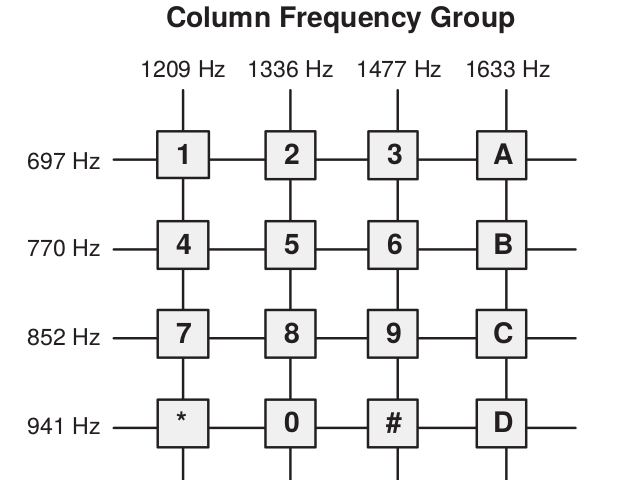
\includegraphics[width=0.5\textwidth]{DTMF_freq}
\caption{DTMF Frequenzen}
\label{fig:DTMF_freq}
\end{figure}
\newline
Der Scalingfaktor lässt sich mit folgender Formel berechnen:
\begin{equation*}\label{eq:Scalingfakt}
	Scalingfaktor = \frac{2*(2^{15}-1)}{f_{sample}}*2^{11}
\end{equation*}
Bei einer Samplingfrequenz von 8000Hz ergibt dies einen Wert von 16777. Wichtig ist hier, dass man den Wert als long speichert (16777L). 

\subsection{ToDo 2}
Beim Todo 2 mussten die Goertzel-Koeffizienten im $Q_{15}$-Format für die jeweilige Frequenz berechnet werden.
\begin{equation*}\label{eq:Goertzel_Koeff}
	\frac{a_k}{2}= \cos(2*\pi*\frac{f_k}{f_s})*2^{15}
\end{equation*}
Auch hier beträgt die Abtastfrequenz 8000Hz und $f_k$ ist die jeweilige Signalfrequenz.

\subsection{ToDo 3}
Die Reihenfolge der Zugriffe muss ein wenig umstrukturiert werden. Zuerst wird das Produkt berechnet und der alte Wert delay[2] abgezogen werden. Anschliessend wird der delay Wert um eins geschoben und der neue Wert berechnet und an der Stelle delay[1] abgelegt. 
\begin{lstlisting}
void goertzel_filter_v1 ( short int * delay, short int input, short int coefficient ){
	
	short int product;
	product = (short int) (( (long) delay[1] * coefficient ) >> 14) - delay[2];

	/* The input is divided by 128 to prevent overload */
	delay[2] = delay[1];
	delay[1] = (short int)( (input >> 7) + product);
}
\end{lstlisting}

\subsection{ToDo 4}
Um den goertzel\_output\_power\_v1 zu berchenen wird der Twiddle-Factor in Realteil und Imaginärteil benötigt. Dieser wird mittels zweier Argumente, in Q15 Format, an die Funktion Übergeben. Die beiden Argumente werden nach Figure 4.17 im DSVB Skript wie folgt berchnet.

\begin{align*}
	&twiddlefactor = W^{k}_{N} \\
	&f_k = k\frac{fs}{N} \\\\
	&b_{RE} =\Re{(-W^{k}_{N})} = \Re{(-e^{-j*2\pi \frac{k}{N}})}=  \Re{(-e^{-j*2\pi \frac{f_k}{f_s}})}\\
	&b_{RE} = -cos(2\pi\frac{f_k}{f_s})\\\\
	&b_{IM} =\Im{(-W^{k}_{N})} = \Im{(-e^{-j*2\pi \frac{k}{N}})}=  \Im{(-e^{-j*2\pi \frac{f_k}{f_s}})}\\
	&b_{IM} = -sin(2\pi\frac{f_k}{f_s})
\end{align*}
\\
Mit $f_k = DTMF$ und $f_s = 8kHz$.
\\
Um das die Werte in das gewünschte Format zubringen wird mit $2^{15}$ multipiziert und das Zweierkomplement gebildet, da keine neagativen Zahlen verwendet werden dürfen. Dies geschiet am einfachsten mit einer Addition von 0xFFFF.

\subsection{ToDo 5}
Diese Berechnung entspricht der Grafik(4.17), ohne die Skalierung um den Faktor $\frac{2}{N^2}$.
\begin{lstlisting}
short int goertzel_output_power_v1(short int * delay, short int b_RE, short int b_IM)
{
	signed int goertzel_power;
	long real;
	long imag;

	real = delay[1] + (b_RE+delay[1]>>15);
	imag = (delay[1]*b_IM)>>15;

	goertzel_power = real*real + imag*imag;

    /* Re-initialize delay. Also useful in event of instability */
	delay[1] = 0;
	delay[2] = 0;

	return goertzel_power;
}
\end{lstlisting}
\end{document}
